% Options for packages loaded elsewhere
\PassOptionsToPackage{unicode}{hyperref}
\PassOptionsToPackage{hyphens}{url}
%
\documentclass[
]{article}
\usepackage{lmodern}
\usepackage{amssymb,amsmath}
\usepackage{ifxetex,ifluatex}
\ifnum 0\ifxetex 1\fi\ifluatex 1\fi=0 % if pdftex
  \usepackage[T1]{fontenc}
  \usepackage[utf8]{inputenc}
  \usepackage{textcomp} % provide euro and other symbols
\else % if luatex or xetex
  \usepackage{unicode-math}
  \defaultfontfeatures{Scale=MatchLowercase}
  \defaultfontfeatures[\rmfamily]{Ligatures=TeX,Scale=1}
\fi
% Use upquote if available, for straight quotes in verbatim environments
\IfFileExists{upquote.sty}{\usepackage{upquote}}{}
\IfFileExists{microtype.sty}{% use microtype if available
  \usepackage[]{microtype}
  \UseMicrotypeSet[protrusion]{basicmath} % disable protrusion for tt fonts
}{}
\makeatletter
\@ifundefined{KOMAClassName}{% if non-KOMA class
  \IfFileExists{parskip.sty}{%
    \usepackage{parskip}
  }{% else
    \setlength{\parindent}{0pt}
    \setlength{\parskip}{6pt plus 2pt minus 1pt}}
}{% if KOMA class
  \KOMAoptions{parskip=half}}
\makeatother
\usepackage{xcolor}
\IfFileExists{xurl.sty}{\usepackage{xurl}}{} % add URL line breaks if available
\IfFileExists{bookmark.sty}{\usepackage{bookmark}}{\usepackage{hyperref}}
\hypersetup{
  pdftitle={Climate Change},
  pdfauthor={null},
  hidelinks,
  pdfcreator={LaTeX via pandoc}}
\urlstyle{same} % disable monospaced font for URLs
\usepackage[margin=1in]{geometry}
\usepackage{graphicx,grffile}
\makeatletter
\def\maxwidth{\ifdim\Gin@nat@width>\linewidth\linewidth\else\Gin@nat@width\fi}
\def\maxheight{\ifdim\Gin@nat@height>\textheight\textheight\else\Gin@nat@height\fi}
\makeatother
% Scale images if necessary, so that they will not overflow the page
% margins by default, and it is still possible to overwrite the defaults
% using explicit options in \includegraphics[width, height, ...]{}
\setkeys{Gin}{width=\maxwidth,height=\maxheight,keepaspectratio}
% Set default figure placement to htbp
\makeatletter
\def\fps@figure{htbp}
\makeatother
\setlength{\emergencystretch}{3em} % prevent overfull lines
\providecommand{\tightlist}{%
  \setlength{\itemsep}{0pt}\setlength{\parskip}{0pt}}
\setcounter{secnumdepth}{-\maxdimen} % remove section numbering

\title{Climate Change}
\author{null}
\date{null}

\begin{document}
\maketitle

{
\setcounter{tocdepth}{4}
\tableofcontents
}
\emph{Working, needs graphics to break up text, formatting for
consistency, link to (existing) short videos that summarize some
content?}

\hypertarget{climate-change-and-stsm-modeling}{%
\subsection{Climate Change and STSM
Modeling}\label{climate-change-and-stsm-modeling}}

The goal of this section is to help you identify questions that the
LANDFIRE BpS models, with their built-in simplifications, strengths, and
constraints, are best suited to help you explore.

\hypertarget{background}{%
\subsubsection{Background}\label{background}}

Directional changes in climate factors, such as \textbf{increases in
minimum or maximum temperatures, changes in precipitation patterns, and
increases in evaporation and transpiration rates,} are influencing
vegetation dynamics through many mechanisms operating at a range of
scales, from genes to biomes. Observed changes, in addition to
ecological theory, allow us to generate hypotheses on how these changes
may play out. As noted in a {[}previous sections{]} (link to Modeling
perspectives), all models are a simplification of reality, and there are
many different aspects of climate change that you might be interested in
exploring with a model.

Climate drivers like \textbf{temperature} and \textbf{moisture
availability} play critical roles in shaping the life history of plants
and associated species in terrestrial ecosystems. As anthropogenic
factors have acted to accelerate the rate of climate change, we are
seeing a wide array of responses in plants, and other species that
strongly influence vegetation dynamics.

\begin{quote}
The most frequently documented responses to climate change include
changes in phenology (the timing of seasonal events, such as budburst),
spatial shifts in range boundaries, and shifts in density patterns
within a species' range due to changes in recruitment or mortality as
site conditions change.
\end{quote}

Given that over evolutionary time, each species has developed a set of
traits that reflect climate, abiotic factors, and competition for
resources and other types of species interactions, we expect that the
suite of species that make up an ecosystem will not all respond in the
same way, leading to shifts in plant community composition.

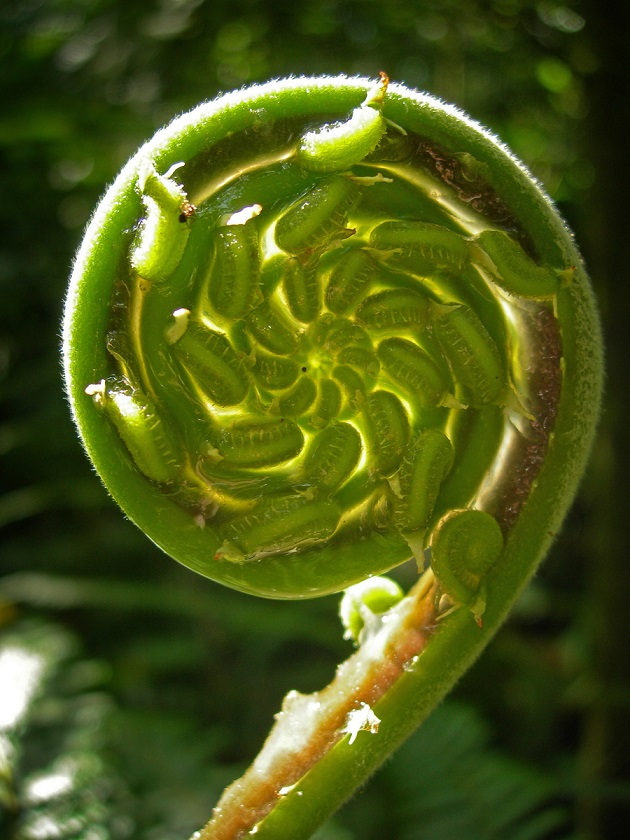
\includegraphics[width=0.45\linewidth]{images/fern}

Photo: © Marci Eggers, TNC. Close-up of of fern about to spring open in
the Atlantic Forest rainforest, Guaraquecaba, Brazil.

\begin{blue}

Notably for applications with BpS models, changes in climate are
influencing disturbance regimes. For example:

\begin{enumerate}
\def\labelenumi{\arabic{enumi}.}
\item
  Drought tends to lengthen fire seasons and increase fire intensity
\item
  Higher temperatures (or temperature gradients) increase the intensity
  and dominant direction of wind patterns and probability of severe
  storms (i.e.~hurricanes)
\item
  Increasing temperatures strongly affect poikilothermic (cold-blooded)
  species associated with vegetation, contributing to increased growth
  rates and higher numbers of generations per growing season for
  leaf/sap consuming insects
\end{enumerate}

\end{blue}

\hypertarget{climate-change-and-bps-models}{%
\subsection{Climate change and BpS
models}\label{climate-change-and-bps-models}}

As described here (link to a section on model structure), LANDFIRE BpS
models are comprised of a set of states and transitions. Each state is a
recognizable seral stage or ``condition'' of a particular vegetation
type, and these states are linked by deterministic transitions (usually
representing growth towards an older, taller age class), and stochastic
transitions representing disturbances such as fire (with an associated
probability land intensity), windthrow, insect outbreak, etc. These
transitions describe how one vegetation state is changed to a different
state. In the montane sagebrush steppe ecosystem example below, the
dominant species is ``X'' and the growth and response to disturbances
are reflected in that species' biology. Common to this ecosystem would
be disturbances such as wildfire and invasive species (i.e.~cheatgrass).

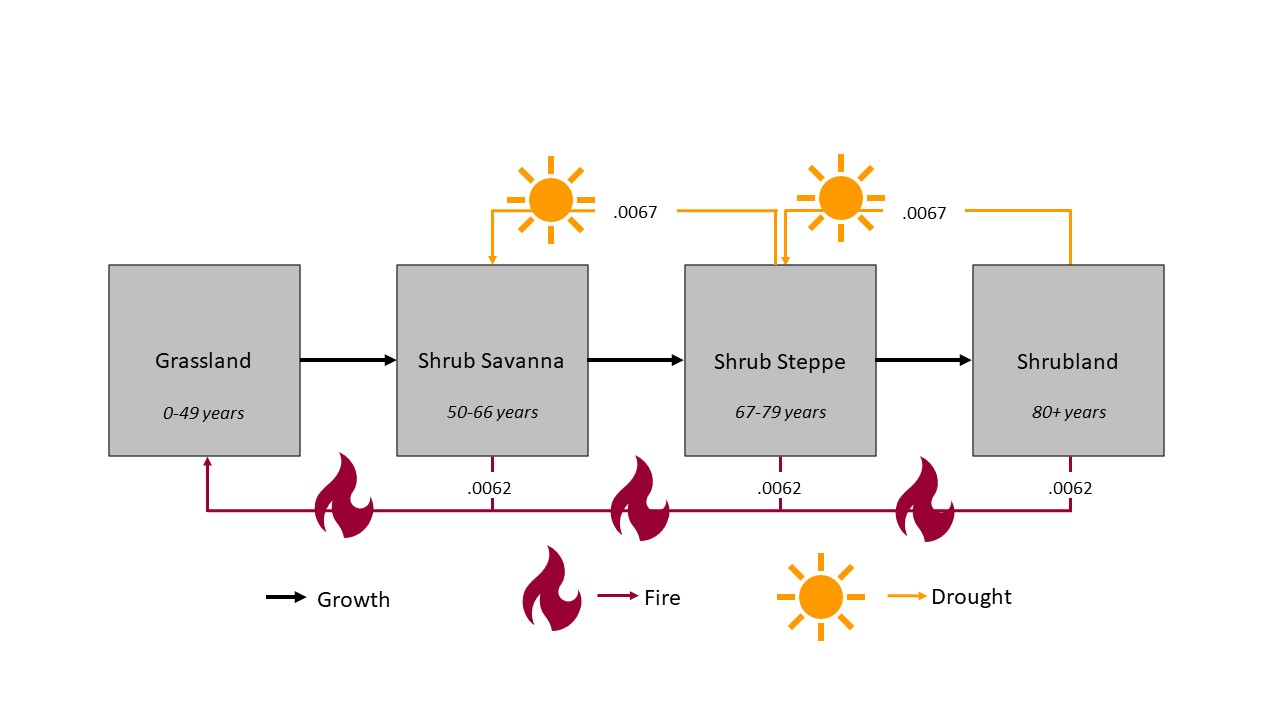
\includegraphics{images/STSMex.jpg} In other vegetation classes with
higher tree species diversity, such as mixed hardwood forests of the
southern Appalachians, transitions represent an average across multiple
species that are likely responding to climate drivers in different ways.

\hypertarget{changes-in-disturbance-regime}{%
\subsection{Changes in disturbance
regime}\label{changes-in-disturbance-regime}}

The ``sweet spot'' for LANDFIRE BpS models in a climate change context
is exploring \textbf{how climate change can influence disturbance
regimes,} and as a result influence the relative proportion of each
ecosystem state over time. These tools allow users to consider time
periods much longer than human experience (i.e., hundreds or thousands
of years) and ``illuminate'' (link to Jim's overview) how events with a
range of different frequencies can interact to shape the distribution of
vegetation classes on the landscape. However, remember that while the
impacts of climate change on ecological systems are complex, this does
not mean you should try to capture the full range of complexity in your
model.

For example, the interaction between \textbf{drought}, \textbf{insect
outbreaks}, and \textbf{fire} is an example of a multi-factor,
climate-related driver of change in forested ecosystem, especially
notable now in the western U.S.

\begin{quote}
While you could take an existing BpS model and add a drought factor,
modify the current fire disturbances, and add an insect pest factor, if
in effect these three drivers tend to operate together, we suggest at
least starting your modeling work by treating this complex of drivers as
\textbf{one disturbance}, potentially starting with the one for which
you have the best information on rates (this might be fire regime).
\end{quote}

\textbf{Placeholder: insert slide with insect invasion added, and
possible more perturbations introduced OR reflective of the fire regime
comment}

As you gain experience and insight, you can consider what additional
things you might learn by trying to tease apart these interacting
factors -- for example by bringing in insect outbreaks as a separate
factor, but with rates that recognize the role of drought conditions in
both disturbance pathways (fire and insects). In the bulleted sections
below, we link climate-related changes to how you would model them in
the BpS-in-SyncroSim platform, moving from the basics to more specific
hypotheses of change.

\hypertarget{altering-disturbances}{%
\subsubsection{Altering disturbances}\label{altering-disturbances}}

\begin{itemize}
\tightlist
\item
  Adding or removing a type of disturbance (see below)
\item
  Modifying the intensity, or distribution across intensity levels
  (e.g., low, med, high)
\item
  Changing the rate (probability) -- with the caveat that the models are
  aspatial, so if spread of the disturbance across the landscape is a
  process you want to understand, you will likely want to complement
  your work with additional tools
\item
  Incorporating a rate multiplier, which allows the probability of a
  disturbance to change over time
\end{itemize}

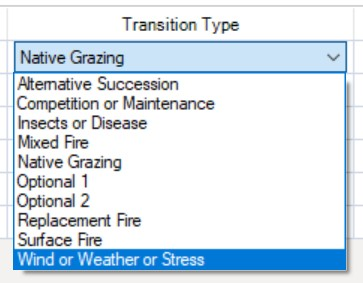
\includegraphics[width=0.35\linewidth]{images/disturbance}

\hypertarget{altering-states}{%
\subsubsection{Altering states}\label{altering-states}}

\begin{itemize}
\tightlist
\item
  Adding or removing vegetation classes. This can include adding a new
  invasive plant species that is favored by some aspect of climate
  change.
\item
  Slowing down or speeding up succession to represent a change in growth
  rates, or slower recovery (see above).
\item
  Transitioning a vegetation class to a new BpS (? Not sure you want
  this here??)
\end{itemize}

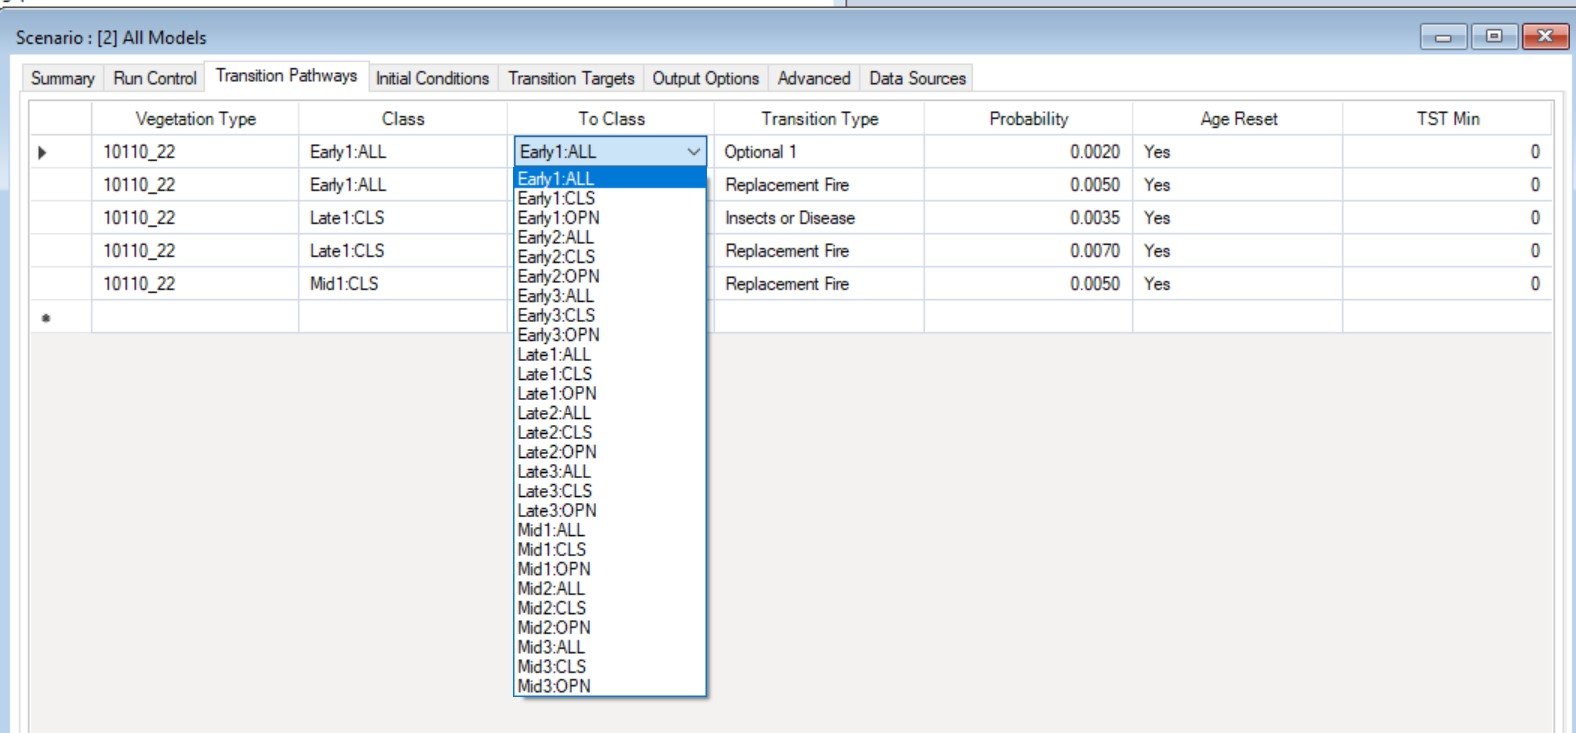
\includegraphics[width=1\linewidth]{images/states}

\hypertarget{bps-and-climate-change-examples}{%
\subsection{BpS and climate change
examples}\label{bps-and-climate-change-examples}}

\hypertarget{more-intense-fires}{%
\paragraph{More intense fires}\label{more-intense-fires}}

Increases in the intensity of fires, a trend that has been observed in
forests with high vegetation density, often in combination with drought.
To represent this process, you would \textbf{increase the probablility
of high intensity fires} in your model -- or potentially add this type
of disturbance if it was not already in the model.

\hypertarget{longer-fire-seasons}{%
\paragraph{Longer fire seasons}\label{longer-fire-seasons}}

\begin{itemize}
\tightlist
\item
  \href{https://doi.org/10.1111/geb.13058}{Cattau et al.~2020} examine
  the extension of the duration of the fire season due to climate change
  both by natural ignition sources and human-caused fires. Looking at
  this question would involve \textbf{increasing the fire return
  interval} within this modeling platform.
\end{itemize}

\hypertarget{larger-fires}{%
\paragraph{Larger fires}\label{larger-fires}}

\begin{itemize}
\tightlist
\item
  Similarly, increasing the spatial extent of fires -- mechanistically,
  this also involves increasing the rate of fires, so it's hard to
  separate the two mechanism of change using the LANDFIRE BpS model.
\end{itemize}

\hypertarget{insect-outbreaks}{%
\paragraph{Insect outbreaks}\label{insect-outbreaks}}

\begin{itemize}
\item
  Insect outbreaks that promote a state change in vegetation are not
  included in the ``out of the box'' BpS models. \textbf{Insect
  outbreaks can be added, and then varied, in all of the ways described
  above for fire.}

  Warming temperatures:

  \begin{itemize}
  \tightlist
  \item
    increase the overwinter survival of insects
  \item
    increase the number of generations possible in a single season
  \item
    increase insect growth rates
  \end{itemize}

  Adding a separate insect outbreak component may be highly relevant,
  especially if there is evidence to support impacts that are
  independent of other drivers. In the case of drought-stressed trees
  contributing to high tree mortality, understanding variations in
  drought risk, for example associated with topography or soil water
  holding capacity, may allow you to partition out impacts by site
  conditions (see last bullet).
\end{itemize}

\hypertarget{transitions-in-vegetation-classes}{%
\paragraph{Transitions in vegetation
classes}\label{transitions-in-vegetation-classes}}

\begin{itemize}
\item
  In some vegetation systems, managers have observed that increases in
  the intensity or extent of fires is leading to a failure of the
  ecological system to regenerate -- reasons may include a loss of
  organic soil horizons in the intense fire, or a lack of seed sources
  close to the newly burned area. This observation could be modeled by
  \textbf{adding a new vegetation class} (perhaps a grass or shrub
  class, if the intent is to explore how this shift might drive an
  ecological transformation), or by \textbf{increasing the duration of
  transition from the post-fire seral stage back to forest}, to
  represent slower regrowth of trees, perhaps aided by active seed
  additions.\\
  Representing variations in climate change exposure, or adaptive
  capacity within an assessment region
\item
  While BpS models are aspatial (see below), you can capture that
  variation by \textbf{developing separate iterations of the same model
  if you have information on how vegetation dynamics might vary within
  an assessment area.} For example, topographic factors or soil moisture
  may strongly influence the sensitivity of a system to a disturbance,
  the rate of recovery after a disturbance, or the probability that a
  disturbance will shift a vegetation type to a new class.
\end{itemize}

\emph{(delete this paragraph?)} The influence of native and non-native
insect pests is changing due to climate change, a pattern that can have
major impacts on forest health when combined with a change in tree
health due to drought exposure. Like fire, changes in the impact of
insects can occur through changes in intensity, and/or duration of
exposure (i.e., warmer temperatures are increasing overwinter

\hypertarget{bps-models-are-not-spatial-models}{%
\subsection{BpS models are not spatial
models}\label{bps-models-are-not-spatial-models}}

The structure of the BpS models provides a clear indication of the
ecological level at which they operate, and can be applied to address
questions about climate change. While range shifts are some of the most
studied aspects of climate change responses, these models are not
spatial, and tend to ``lump'' all species within a vegetation class
together within a series of states. \textbf{This is because it would be
impossible to use this modeling platform to model the mechanistic
relationships between all species within all types of
ecosystems\ldots{}} If you are interested in exploring vegetation
responses within what the BpS models consider a ``state'' -- for
example, exploring changes in species composition that might occur as a
result of changes in tree competitive ability as growing seasons
lengthen due to a warming climate -- BpS models are likely not the best
hammer for that nail!

\end{document}
